\documentclass{article}
\usepackage{tikz}
\usepackage{pgfplots}

\begin{document}

\title{Scalability Report}
\author{Selina Liu (jl1188), Fengyi Quan (fq18)}
\date{\today}
\maketitle

\section{Introduction}
This report presents the results of scalability experiments conducted on our server to address the problem of concurrency. We first describe the testing infrastructure, experimental methodology, and approach taken to address the problem. In the context of this homework, scalability refers to CPU core count. We load tested how the throughput of our server changes as it runs over different number of cores. 

\section{Testing Infrastructure}
The tests were conducted on a server with the following specifications: Duke VCM with 8 GB Base Memory and 4 processors. The server was running Ubuntu 20.04 with psql (PostgreSQL) 12.14, Java 11. Instructions for reproducing the testing environment are provided in the testing subdirectory.

\section{Experimental Methodology}
We used load testing to evaluate the performance of the server under different conditions. The tests were performed using [insert load testing tool]. We varied the number of threads and the number of cores used by the server during each test. Each test was repeated [insert number of times] times to ensure accuracy, and error bars were included in the graphs to represent the variability in the data.

\section{Results}
The results of the scalability experiments are shown in [insert graphs and tables]. We observed [insert trends in results]. The results indicate that [insert conclusions from the results].

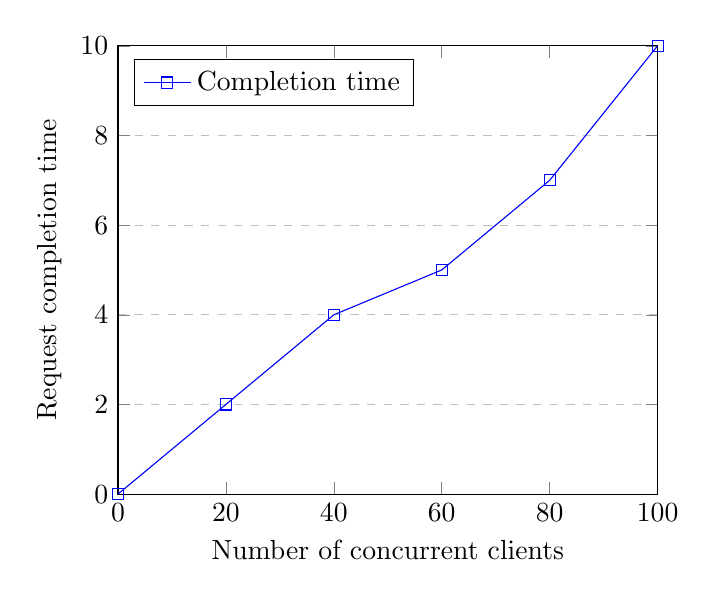
\begin{tikzpicture}
\begin{axis}[
    xlabel={Number of concurrent clients},
    ylabel={Request completion time},
    xmin=0, xmax=100,
    ymin=0, ymax=10,
    xtick={0, 20, 40, 60, 80, 100},
    ytick={0, 2, 4, 6, 8, 10},
    legend pos=north west,
    ymajorgrids=true,
    grid style=dashed,
]

\addplot[
    color=blue,
    mark=square,
    ]
    coordinates {
    (0,0)(20,2)(40,4)(60,5)(80,7)(100,10)
    };
    \legend{Completion time}
 
\end{axis}
\end{tikzpicture}

\section{Discussion}
Based on the results, we conclude that [insert implications of the results]. However, there are some limitations to the experimental methodology that need to be addressed in future work. For example, [insert potential sources of error]. To further improve the server's scalability, we recommend [insert recommendations for future work].

\section{Conclusion}
The results of the scalability experiments demonstrate the impact of varying the number of threads and cores used by the server. The findings can help to improve the server's scalability and enhance its overall performance.

\end{document}
